\section{Distribution of Predicted Gene Lengths}

To better understand and compare the distributions of gene lengths
predicted by Braker2, GeneMark, and RefSeq, the cumulative density
function for the lengths of CDS sequences for each gene finding tool
are shown in figure ~\ref{fig:cdf-lengths}. The $\log_{10}$ values of
gene lengths were used for a better visulazation of the
distributions. In DC1, the curves from Braker2 and GeneMark follow
each other closely, with the only variation being genes of short
length, where Braker2's curve extends beyond that of GeneMark,
indicating that Braker2 predicts more shorter genes than GeneMark. In
the case of Tsth20, the curves are nearly identical. In
\textit{T. reesei}, we see disagreement in the curves for shorter
genes, with Braker2 appearing to predict a greater amount of shorter
genes than GeneMark and RefSeq. The upper portions of the curves trend
toward similar predicted gene lengths. In \textit{T. harzianum},
RefSeq deviates from GeneMark and Braker2, predicting more genes of
short length, while Braker and GeneMark appear to be in near-complete
agreement. Finally, in \textit{T. virens}, we see the RefSeq curve
predicting shorter genes once again, although the deviation is not as
drastic as in \textit{T. harzianum}. From these plots, we can say that
visually, gene finding tools appear to predict different lengths of
genes. We also observe that Braker2 predicts the shortest genes of all
three gene finding methods.

\begin{figure}[p!]
  \centering
  \begin{subfigure}{0.7\textwidth}
    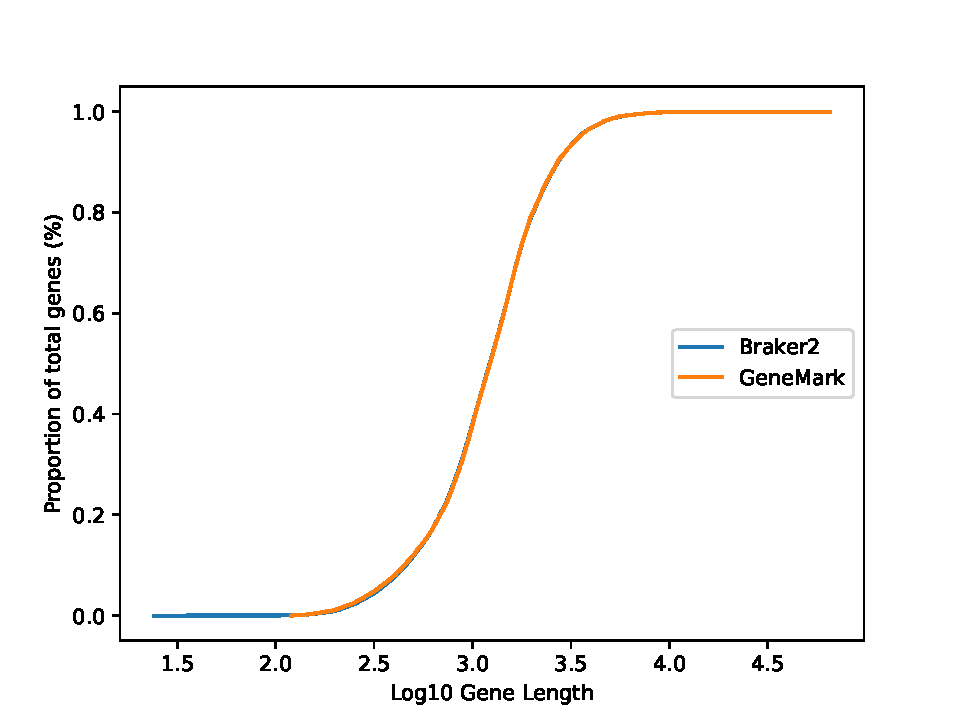
\includegraphics[width=\textwidth]{figures/dc1-cdf-lengths-log.pdf}
    \label{fig:dc1-lengths}
    \caption{DC1}
  \end{subfigure}
  \begin{subfigure}{0.7\textwidth}
    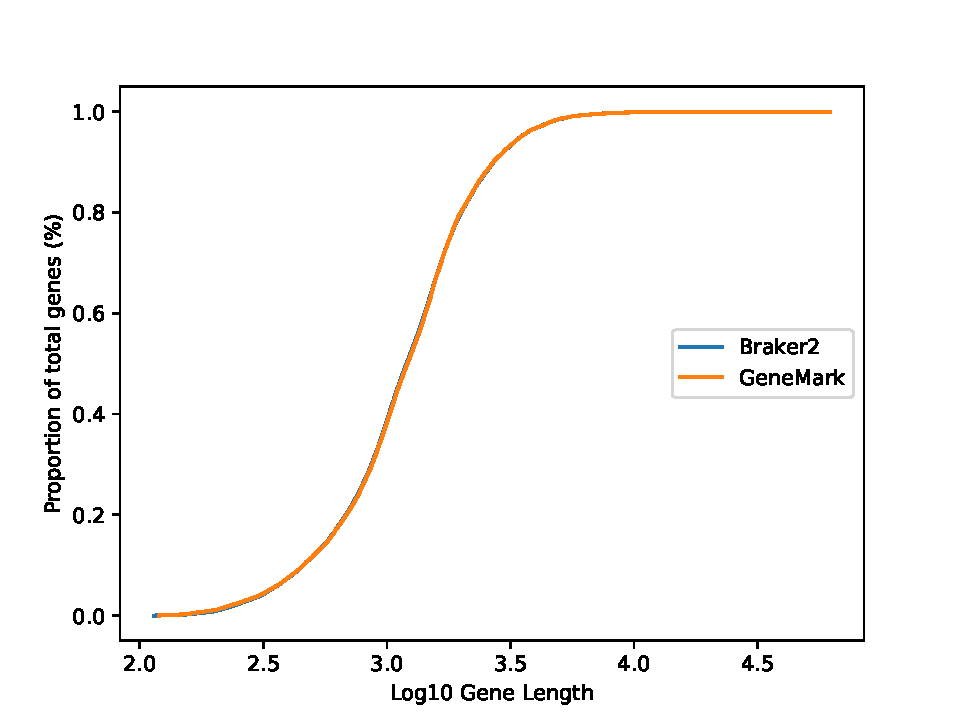
\includegraphics[width=\textwidth]{figures/tsth20-cdf-lengths-log.pdf}
    \label{fig:tsth20-lengths}
    \caption{Tsth20}
  \end{subfigure}
\end{figure}
\begin{figure}[p!]
  \ContinuedFloat
  \centering
  \begin{subfigure}{0.7\textwidth}
    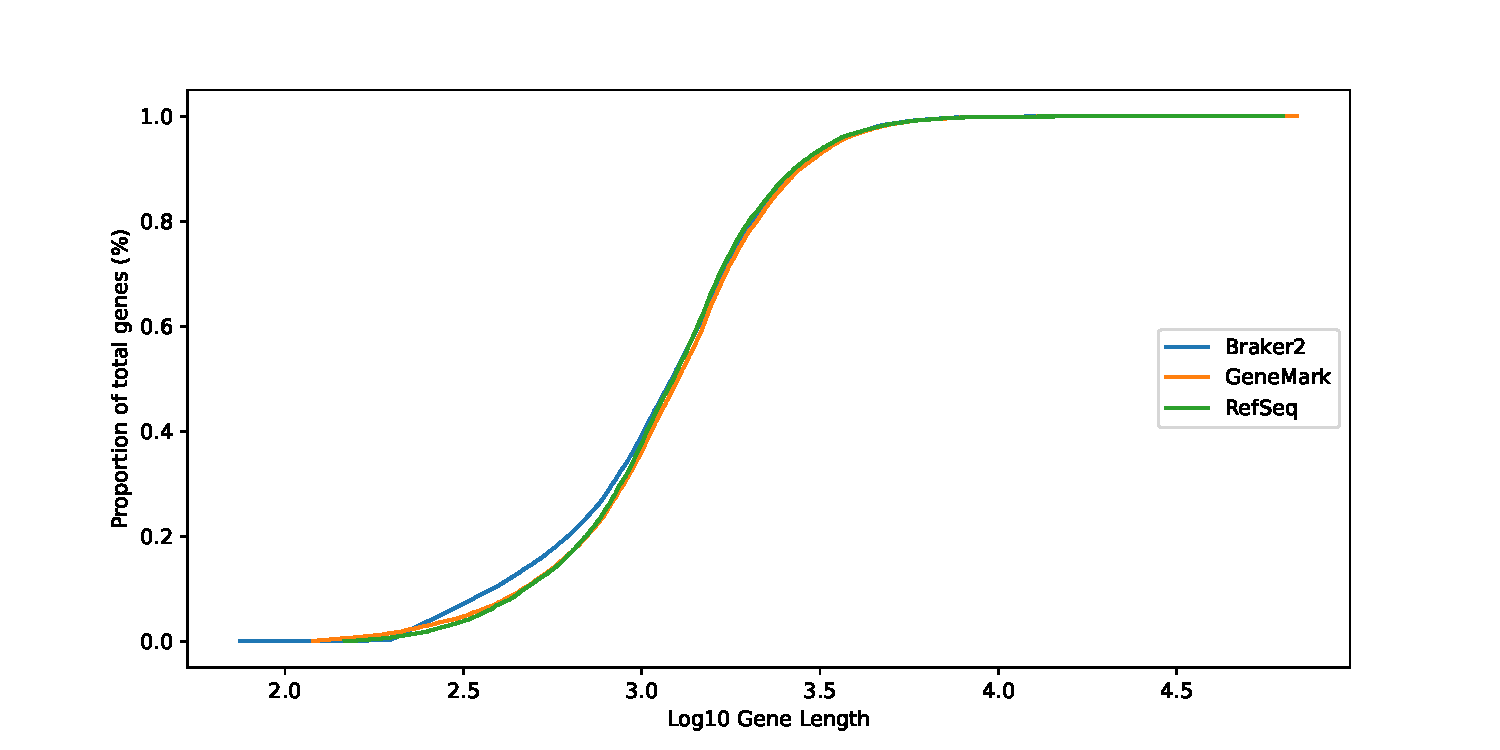
\includegraphics[width=\textwidth]{figures/t-reesei-cdf-lengths-log.pdf}
    \label{fig:treesei-lengths}
    \caption{\textit{T. reesei}}
  \end{subfigure}
  \begin{subfigure}{0.7\textwidth}
    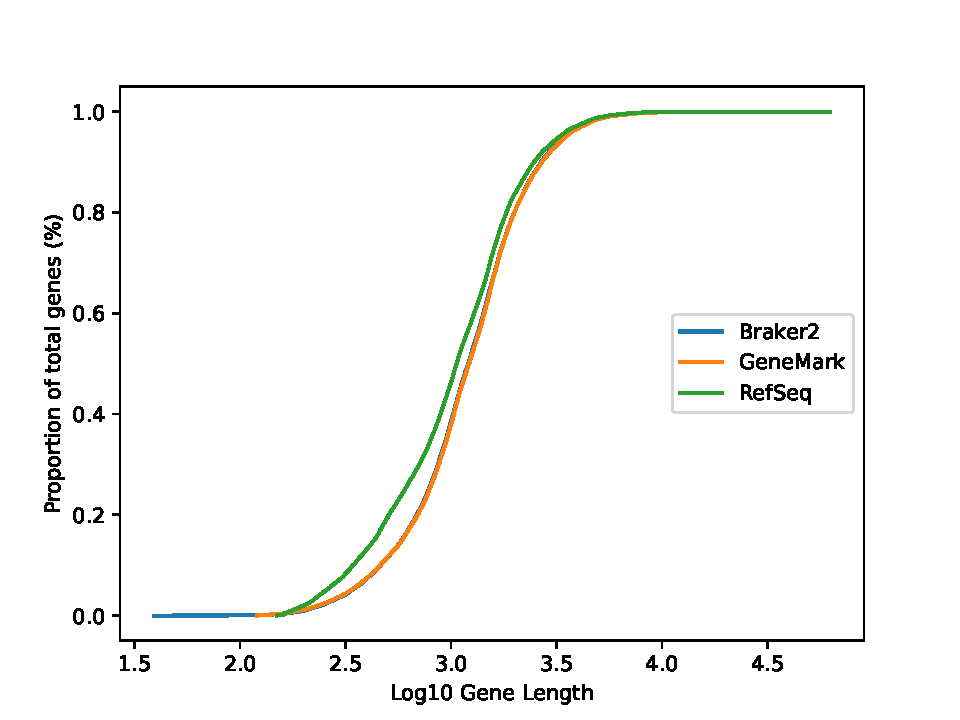
\includegraphics[width=\textwidth]{figures/t-harzianum-cdf-lengths-log.pdf}
    \label{fig:tharzianum-lengths}
    \caption{\textit{T. harzianum}}
  \end{subfigure}
\end{figure}
\begin{figure}[p!]
  \ContinuedFloat
  \centering
  \begin{subfigure}{0.7\textwidth}
    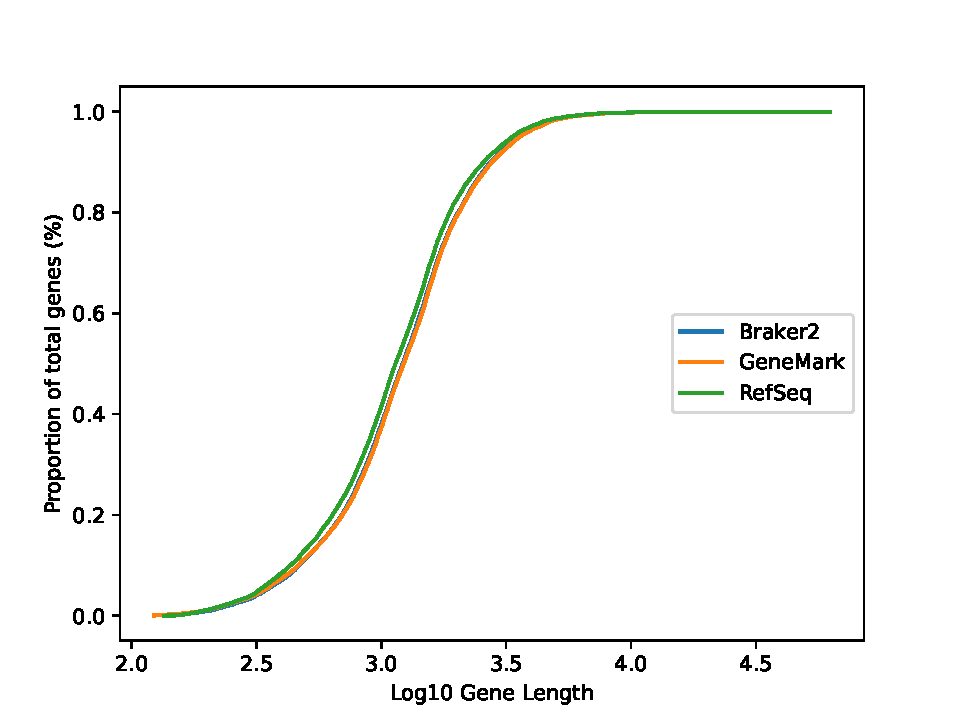
\includegraphics[width=\textwidth]{figures/t-virens-cdf-lengths-log.pdf}
    \label{fig:tvirens-lengths}
    \caption{\textit{T. virens}}
  \end{subfigure}
  \caption[Cumulative Density Function of Gene Lengths]{Plots of the
    cumulative density function for CDS lengths predicted by each gene
    finding tool.}
  \label{fig:cdf-lengths}
\end{figure}

To confirm these observations statistically, two-sided two-sample
Kolmogorov-Smirnov tests were performed using the $\log_{10}$
transformed gene lengths and are presented in table
\ref{table:ks-2s}. In the cases of DC1 and Tsth20, we see that Braker2
and GeneMark do not produce statistically different lengths of genes,
which is interesting considering that the Braker2 includes
experimental evidence for another assembly while GeneMark does not. In
\textit{T. reesei}, while RefSeq and GeneMark do not reject the null
hypothesis when compared, Braker2's predicted gene lengths are
significantly different than both RefSeq and GeneMark, which is also
confirmed visually in the CDF plots above. The same cannot be said for
\textit{T. harzianum} and \textit{T. virens}, where RefSeq is
significantly different from both GeneMark and Braker2, which are not
significantly different from eachother. It is also notable that RefSeq
and GeneMark predict similar gene lengths in \textit{T. reesei} but
not in \textit{T. harzianum} and \textit{T. virens.}

\begin{table}
  \begin{center}
    \begin{tabular}{|c|c|c|c|c|c|c|}
      \hline
      Genome & Tool \#1 & Tool \#2 & \textit{P}-value  \\ \hline
      DC1 & Braker2 & GeneMark & $0.999$ \\ \hline
      Tsth20 & Braker2 & GeneMark & $0.965$ \\ \hline
      \textit{T. reesei} & Braker2 & GeneMark & $9.481^{-07}$ \\ \hline
      \textit{T. reesei} & GeneMark & RefSeq & $0.002$ \\ \hline
      \textit{T. reesei} & Braker2 & RefSeq & $1.340^{-07}$ \\ \hline
      \textit{T. harzianum} & Braker2 & GeneMark & $0.863$ \\ \hline
      \textit{T. harzianum} & GeneMark & RefSeq & $4.313^{-52}$ \\ \hline
      \textit{T. harzianum} & Braker2 & RefSeq & $4.674^{-55}$ \\ \hline
      \textit{T. virens} & Braker2 & GeneMark & $0.635$ \\ \hline
      \textit{T. virens} & GeneMark & RefSeq & $7.352^{-12}$ \\ \hline
      \textit{T. virens} & Braker2 & RefSeq & $1.794^{-09}$ \\ \hline
    \end{tabular}
  \end{center}
  \caption{Table of \textit{P}-values from two-sided two-sample
    Kolmogorov-Smirnov tests between gene finding tools.}
  \label{table:ks-2s}
\end{table}

It can clearly be stated that these gene finding tools predict
different lengths of genes, paritcularly in \textit{T. reesei,
  harzianum} \textit{T. virens}. Why that may be the case is difficult
to answer without deeper invesitgation. There is clearly an underlying
difference between the gene finding tools, in particular when training
data is introduced. We observe that when gene finders are applied to
the assemblies from which their training data originated, they tend to
predict shorter genes. Conversly, we observe that when a gene finding
tool trained with experimental evidence is applied to a different
\textit{Trichoderma} assembly, the lengths of predicted genes do not
significantly differ from an \textit{ab initio} gene finder like
GeneMark, except in the case of RefSeq's predictions on
\textit{T. reesei}.
